\chapter{Rekurrente Netze}
\section{Modelle von Rekurrenten Netzen}
Wie in der Einleitung bereits erw�hnt, k�nnen die Architekturen eines rekurrenten Netzes viele verschiedene Formen annehmen. In diesem Kapitel werden zwei Modelle beschrieben, das Input-Output Model und das State-Space Model.\cite{haykin}

\subsection{Input-Output Model}
\begin{figure}[H]
	\centering
	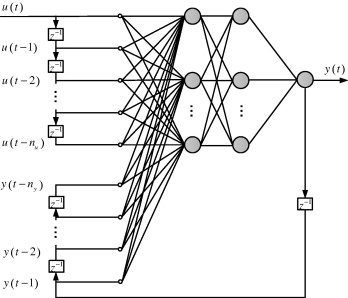
\includegraphics[height=8cm]{narx.jpg}
	\caption{Input-Output Model \itshape(sciencedirect.com)\upshape}
	\label{iomodel}
\end{figure}
Abbildung \ref{iomodel} zeigt eine Architektur eines rekurrenten Netzes mit einem einzelnen Inputsignal $u(t)$ mit einer Zeitverschiebung von $n_u$ Einheiten. Au�erdem hat es ein Outputsignal $y(t)$, welches �ber $n_y$ Zeitverschiebungen wieder als Input verwendet wird. Ein solches Modell nennt man Input-Output Model.\\
Dadurch ergeben sich folgende Inputdaten f�r das Netz:
\begin{itemize}
	\item Die akutellen und die vergangenen Inputwerte $u(t), u(t-1),\ldots,u(t-n_u)$
	\item und die zeitverz�gerten Werte des Outputneurons $y(t-1),\ldots,y(t-n_y)$.
\end{itemize}
Ein solches Modell besitzt ein dynamsiches Verhalten welches durch
$$y(t) = F\left(y(t-1),\ldots,y(t-n_y),u(t),\ldots,u(t-n_u)\right)$$
beschrieben wird, wobei $F$ eine lineare Funktion ist.

\subsection{State-Space Model}
\begin{figure}[H]
	\centering
	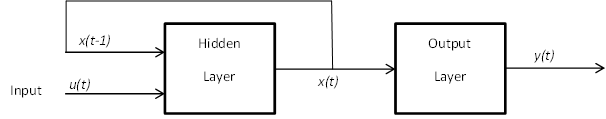
\includegraphics[width=12cm]{StateSpace.png}
	\caption{State-Space Model}
	\label{ssmodel}
\end{figure}
Abbildung \ref{ssmodel} zeigt eine weitere Architektur eines rekurrenten Netzes, welches State-Space Model genannt wird. Dabei wird der Output der verdeckten Schicht $x(t)$ zeitversetzt wieder zum Input dazugenommen. Der Input besteht also aus einer Verkettung der Inputwerte $u(t)$ und den zeitversetzten Outputwerten der verdeckten Schicht. Auch hier k�nnen mehrere zeitversetzte Werte der Input- beziehungsweise der verdeckten Schicht verwendet werden. Somit erhalten wir ein dynamisches Verhalten des State-Space Model mit der Gleichung
\begin{align*}
	x(t) &= f\left(x(t-1),u(t)\right) \text{ und}\\
	y(t) &= C x(t),
\end{align*}
wobei $f$ eine lineare Funktion und $C$ die Gewichte zur Outputschicht darstellen.\\

Beide Modelle lassen sich durch ein Elman Netz darstellen.
